\begin{figure}
	\centering
  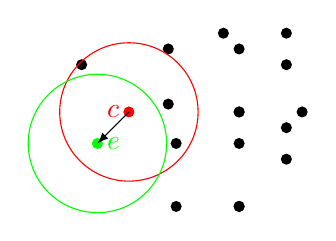
\begin{tikzpicture}
		\fill (-2,1.8) circle(2pt);
		\fill (-.9, 1.3) circle(2pt);
		\fill (-.9,2) circle(2pt);
		\fill (-.8,.8) circle(2pt);
		\fill (-.8,0) circle(2pt);
		\fill (-.2,2.2) circle(2pt);
		\fill (0,0) circle(2pt);
		\fill (0,1.2) circle(2pt);
		\fill (0,1.2) circle(2pt);
		\fill (0,0) circle(2pt);
		\fill (0,.8) circle(2pt);
		\fill (0,2) circle(2pt);
		\fill (.6,1) circle(2pt);
		\fill (.6,.6) circle(2pt);
		\fill (.6,1.8) circle(2pt);
		\fill (.6,2.2) circle(2pt);
		\fill (.8,1.2) circle(2pt);
    
    \fill[red] (-1.4,1.2) circle(2pt) node[anchor=east]{$ c $};
    \draw[red] (-1.4,1.2) circle(25pt);
    
    \fill[green] (-1.8,.8) circle(2pt) node[anchor=west]{$ e $};
    \draw[green] (-1.8,.8) circle(25pt);
    
		\draw[-latex] (-1.4,1.2) -- (-1.8,.8);
		
  \end{tikzpicture}
  \caption{Punkt rdzeniowy $ c $, brzegowy $ e $ oraz relacja bezpośredniego zasięgu gęstościowego $ dirreach_{\varepsilon,\mu}(e, c) $, $ \mu=3$.}\label{fig:core-edge-point}
\end{figure}